\section{Schéma de la démonstration du paradoxe de Hausdorff.}
\noindent
Dans cette section on présente une vue d'ensemble de la démonstration du paradoxe de Hausdorff, avant de s'atteler aux détails de la démonstration.
Les raisonnements de cette section sont inspirés de la réference \cite{cite2}.
Avant de lister les étapes qu'on va suivre, on a tout d'abord besoin de quelques définitions
\begin{definition}
  Un alphabet dans un ensemble $\mathrm{G}$ est un ensemble fini et non vide d'éléments distincts de $\mathrm{G}$.
\end{definition}
\begin{definition}
  Un mot défini dans un alphabet $\mathcal{A}$ est une suite finie d'éléments de $\mathcal{A}$.\\ La longueur d'un tel mot est le nombre d'éléments dans la suite.
\end{definition}
\begin{definition}
Un mot est dit réduit s'il ne contient pas deux éléments consécutifs qui soient inverses l'un de l'autre.
\end{definition}
\begin{definition}
  On dit que deux éléments $\theta$ et $\varphi$ d’un groupe $\mathrm{G}$ sont indépendants si pour tout mot réduit de longueur $n\ge 2$, $(g_1, ..., g_n)$ dans l'alphabet $\mathcal{A} = \{\theta, \varphi, \theta^{-1}, \varphi^{-1}\}$ on a que $g_1...g_n \ne 1_\mathrm{G}$.
\end{definition}
% \begin{definition}
% On dit que deux éléments $\theta$ et $\varphi$ d’un groupe $\mathrm{G}$ sont indépendants si les éléments $\theta$, $\varphi$, $\theta^{-1}$ et $\varphi^{-1}$ de $\mathrm{G}$ sont tous distincts et si pour tout $n > 2$ et pour toute liste d'éléments $(g_1, ..., g_n)$ de $\mathrm{G}$ tous égaux à $\theta$, $\varphi$, $\theta^{-1}$ ou $\varphi^{-1}$, il est impossible d’avoir $g_1...g_n = 1$ si $g_ig_{i+1} \neq 1$ pour $i = 1, ..., n-1$.
% \end{definition}
\begin{definition}
Si un groupe $\mathrm{G}$ est engendré par deux éléments $\theta$ et $\varphi$ indépendants, on dit
que $\mathrm{G}$ est librement engendré par $\theta$ et $\varphi$. $\mathrm{G}$ est alors appelé un groupe libre de rang $2$.
\end{definition}
\noindent
Pour démontrer notre \hyperref[But]{théorème} on va procéder comme suit
\subsection{Première étape de la démonstration .}
% %%%%%%%%%%%%%%%%%%%%%%%%%%%%%%%%%%%%%%%%%%%%%%%%%%%%%%%%%%%%%%%%%%%%%%%%%%%%%%%%%%%%%%%%%%%%%%%%%%%%%%%%%%%%%%%%%%%%%%%%%%%%
\noindent
 On va construire un groupe libre de rang $2$ contenu dans $\mathcal{SO}(3)$ et engendré par deux éléments $\theta$ et $\varphi$. L'interet de cette construction est que ce groupe peut être représenté par la fractale suivante qu'on appelle le graphe de Cayley:
  \begin{figure}[h]
      \centering
      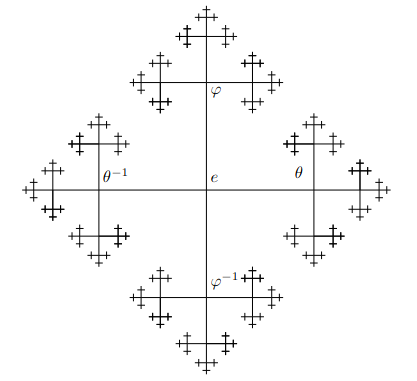
\includegraphics[scale=0.5]{./images/bt.png}
      % \caption{Une représentation graphique d'un groupe libre de rang 2}
      \label{fig1}
  \end{figure}\\
  \noindent
  Dans cette représentation, les éléments de $\mathrm{G}$ sont les intersections des différents segments, et sont répartis de la manière suivante :
  \begin{itemize}
    \item L'élément neutre est le centre de la fractale.
    \item Pour multiplier un élément par $\theta$ à gauche on se déplace (dans la fractale) à partir de cet élément vers la gauche.
    \item Pour multiplier un élément par $\theta^{-1}$ à gauche on se déplace (dans la fractale) à partir de cet élément vers la droite.
    \item Pour multiplier un élément par $\varphi$ à gauche on se déplace (dans la fractale) à partir de cet élément vers le haut.
    \item Pour multiplier un élément par $\varphi^{-1}$ à gauche on se déplace (dans la fractale) à partir de cet élément vers le bas.
  \end{itemize}
  On note $\mathrm{L}(\sigma)$ la composante connexe de la fractale privé de l'élément neutre, qui contient $\sigma$, pour \\$\sigma \in \{\theta, \theta^{-1}, \varphi, \varphi^{-1}\}$.
  Si on multiplie à gauche par $\theta$ la composante $\mathrm{L}(\theta^{-1})$, on obtient la réunion des points des trois composantes $\mathrm{L}(\varphi^{-1})$, $\mathrm{L}(\theta^{-1})$ et $\mathrm{L}(\varphi)$, plus l'élément neutre.\\
\\
  \begin{minipage}{0.1\textwidth}
  \centering
  $\mathrm{L}(\theta^{-1}) =$
  \end{minipage}%
  \begin{minipage}{0.25\textwidth}
  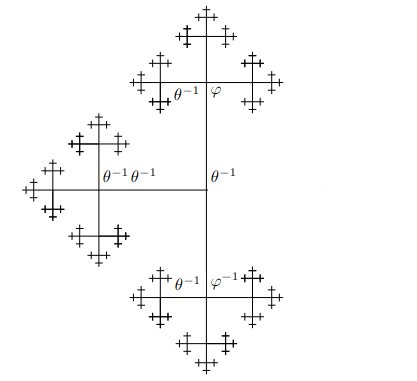
\includegraphics[scale=0.4]{./images/btt.png}
  \end{minipage}%
  \begin{minipage}{0.1\textwidth}
  \centering
  $\overset{\theta}{--\longrightarrow}$ %$\theta\mathrm{L}(\theta^{-1})=$
  \end{minipage}%
  \begin{minipage}{0.25\textwidth}
  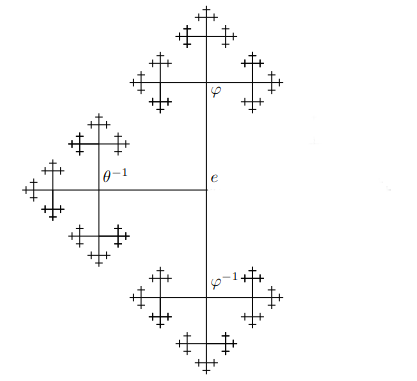
\includegraphics[scale=0.4]{./images/bttt.png}
  \end{minipage}%
  \begin{minipage}{0.3\textwidth}
  \centering
  $=\{e\}\cup \mathrm{L}(\theta^{-1}) \cup \mathrm{L}(\varphi^{-1}) \cup \mathrm{L}(\varphi)$
  \end{minipage}%
\\
\bigskip

\noindent
  De même si on multiplie à gauche par $\varphi$ la composante $\mathrm{L}(\varphi^{-1})$, on obtient les trois composantes $\mathrm{L}(\varphi^{-1})$, $\mathrm{L}(\theta^{-1})$ et $\mathrm{L}(\theta)$, plus l'élément neutre.
  En d'autres termes :
  $$\mathrm{G} = \mathrm{L}(\theta)\cup\theta\mathrm{L}(\theta^{-1})= \mathrm{L}(\varphi)\cup\varphi\mathrm{L}(\varphi^{-1})$$
  % On a pu alors construire $\mathrm{G}$ à partir de parties disjointes dont la réunion est strictement incluse dans $\mathrm{G}$.

  \begin{remarkk}\label{remarque2}
    Le fait que le groupe $G$ est libre implique que ses éléments s'écrivent de manière unique comme mot de l'alphabet $\{\theta, \varphi, \theta^{-1}, \varphi^{-1}\}$; en d'autres mots, on ne peut jamais tomber sur un même élément en partant dans deux chemins différents dans la fractale, et en particulier les réunions ci-dessus sont disjointes.
  \end{remarkk}
  \noindent
  Le groupe $\mathrm{G}$ a donc la propriété d'être décomposable en parties disjointes, $\mathrm{L}(\varphi^{-1})$, $\mathrm{L}(\varphi)$, $\mathrm{L}(\theta^{-1})$ et $\mathrm{L}(\theta)$ telles qu'on peut reconstruire $\mathrm{G}$ soit à partir des deux premières, ou à partir des deux dernières parties.
\subsection{Deuxième étape de la démonstration .}\label{2.}
Après, on va éssayer d'importer cette propriété de $\mathrm{G}$ à $\mathrm{S}^2$ en écrivant $\mathrm{S}^2$ comme réunion d'orbites de $\mathrm{G}$. Ce programme sera mis en difficulté par le fait que la sphère $\mathrm{S}^2$ contient des éléments qui peuvent être fixés par des éléments de $\mathrm{G}$, c.à.d que pour certains $x$ l'application $G \rightarrow S^2$ donnée par $g \rightarrow g(x)$ ne sera pas injective.
  On va donc dans un premier temps travailler avec l'ensemble $$\mathrm{X} = \mathrm{S}^2 - \{s \in \mathrm{S}^2 \mid \exists g \in \mathrm{G}, g(x) = x\}$$ de sorte que l'action de $\mathrm{G}$ sur $\mathrm{X}$ soit libre, i.e :
  \begin{align*}
 g_X \colon X &\to X\\
 x &\mapsto g(x).
\end{align*}
est bijective puisque $g$ est inversible et que :
  \begin{align*}
  \phi \colon \mathrm{G} &\to \mathfrak{S}(X)\\
  g &\mapsto g_X.
\end{align*}
est un homomorphisme qui vérifie que pour tout $x\in X$, $g(x) = x \Rightarrow g = \mathrm{Id_E}$.\\
$G$ a la propriété d'être dans un certain sens algébriquement équidécomposable à deux copies de lui même, on va montrer donc qu'on peut importer cette propriété de $\mathrm{G}$ à $\mathrm{X}$. Pour cela on va procéder comme suit
\begin{itemize}
  \item Dans chaque $G$-orbite de $X$ on va sélectionner un seul élément, pour garantir une unicité des éléments de $X$ après l'action de $G$. Cette selection sera faite en utilisant \hyperref[axiome]{l'axiome du choix}, $M$ sera l'union de ces choix.
  \item On représente donc $\mathrm{X}$ par la même fractale qu'avant, en remplaçant chaque élément $g \in \mathrm{G}$ par l'ensemble $g(\mathrm{M}) \subset \mathrm{X}$. On peut alors répéter le même raisonnement que pour $\mathrm{G}$; en divisant chaque $G$-orbite de la même façon que pour $G$, pour construire $\mathrm{X}$ à partir de parties disjointes dont la réunion est strictement incluse dans $\mathrm{X}$. On dit que $\mathrm{X}$ est \hyperref[ed]{équidécomposable} à deux copies de $\mathrm{X}$.
\end{itemize}
 % En effet, pour garantir une unicité des éléments de $\mathrm{X}$ après l'action de $\mathrm{G}$, on va identifier les éléments $a$ et $b$ de $\mathrm{X}$ qui vérifient $g(a)=h(b)$ pour $g, h \in \mathrm{G}$, et pour cela on va prendre un seul élément de chaque orbite, et donc on utilise \hyperref[axiome]{l'axiome du choix} pour construire un ensemble $\mathrm{M}$ qui contient un représentant de chaque orbite, alors l'ensemble $\mathrm{X}$ peut être représenté par la même fractale qu'avant, sauf à la place de chaque $g \in \mathrm{G}$ on aura $g(\mathrm{M})$, et on peut alors répéter le même raisonnement que pour $\mathrm{G}$ pour construire $\mathrm{X}$ à partir de parties dont l'union est strictement incluse dans $\mathrm{X}$.\\
%   \item \label{2.} Après, on va construire un sous-ensemble $\mathrm{X}$ de $\mathrm{S}^2$ qui à la fois peut être découpée en parties, et réarangée (après rotations et translations) pour obtenir $\mathrm{S}^2$, et tel que l'action de $\mathrm{G}$ sur $\mathrm{X}$ soit libre, i.e :
%   \begin{align*}
%  g_X \colon X &\to X\\
%  x &\mapsto g(x).
% \end{align*}
% est bien définie $\forall g \in \mathrm{G}$ (et même bijective puisque $g$ est inversible) et que :
%   \begin{align*}
%   \phi \colon \mathrm{G} &\to \mathfrak{S}(X)\\
%   g &\mapsto g_X.
% \end{align*}
% soit un homomorphisme qui vérifie que pour tout $x\in X$, $g(x) = x \Rightarrow g = \mathrm{Id_E}$,
%   pour qu'on puisse faire passer la propriété de $\mathrm{G}$ à $\mathrm{X}$.\\ En effet, en utilisant la
%   \hyperref[remarque2]{Remarque 1}, on aurra besoin pour avoir une sorte d'unicité après l'action de $\mathrm{G}$ sur $\mathrm{X}$,
%   qu'aucun élément de $\mathrm{X}$ ne se répète après composition par un élément de $\mathrm{G}$ i.e ,\\ ($\forall x \in X$, $g(x) = x \Rightarrow g = \mathrm{Id_E}$) , de plus il nous faut identifier les éléments $a$ et $b$ de $\mathrm{X}$ qui vérifient $g(a)=h(b)$ pour $g, h \in \mathrm{G}$, et pour cela il nous faut prendre qu'un seul élément de chaque orbite, et donc on utilise l'axiome du choix pour construire un ensemble $\mathrm{M}$ qui contient un représentant de chaque orbite, alors l'ensemble $\mathrm{X}$ peut être représenté par la même fractale qu'avant, sauf à la place des $g$ il y aura des $g(\mathrm{M})$, et on peut alors répéter le même raisonnement que pour $\mathrm{G}$ pour construire $\mathrm{X}$ à partir de parties dont l'union est strictement incluse dans $\mathrm{X}$.\\
%
%   \begin{remarkk}\label{remarque3}
%     Remarquons ici que pour que ce résonnement soit vrai, il ne faut pas que tous les éléments de $\mathrm{X}$ soient regroupés dans le centre de la fractale, c.à.d il faut que $\mathrm{M} \ne \mathrm{X}$, i.e : $\exists x \in \mathrm{X}, \exists g \in G$ tel que $g(x) \ne x$, ce qui est vérifié car l'action est libre.
%   \end{remarkk}
\subsection{Troisième étape de la démonstration .}
\noindent
 En fin, on va montrer que $\mathrm{S}^2$ est \hyperref[ed]{équidécomposable} à $\mathrm{X}$, et donc équidécomposable à la réunion de deux copies de $\mathrm{X}$, et que chaque copie de $\mathrm{X}$ est équidécomposable à $\mathrm{S}^2$, pour conclure que $\mathrm{S}^2$ est équidécomposable à deux copies de $\mathrm{S}^2$.
  % \item En fin, il suffit de transformer $\mathrm{S}^2$ en $\mathrm{X}$, transformer $\mathrm{X}$ en "deux $\mathrm{X}$", et en fin transformer chaqu'un des $\mathrm{X}$ en $\mathrm{S}^2$, (transformer signifie : découper et réaranger après rotations et translations).

%%%%%%%%%%%%%%%%%%%%%%%%%%%%%%%%%%%%%%%%%%%%%%%%%%%%%%%%%%%%%%%%%%%%%%%%%%%%%%%%%%%%%%%%%%%%%%%%%%%%%%%%%%%%%%%%%%%%%%%%%%%%%%%%%%%%%%%%%%%%%
\begin{remarkk}\label{remarque1}
  Un groupe libre de rang $2$ ne peut pas être abélien.($g_1g_2 = g_2g_1 \Rightarrow g_1^{-1}g_2^{-1}g_1g_2=1_G$, ce qui contredit la définition d'un groupe libre).
\end{remarkk}
\noindent
On va chercher donc à construire un sous-groupe libre de rang $2$, $\mathrm{G} = \langle \rho, \tau \rangle$, dans $\mathcal{SO}(3)$. D'après la \hyperref[remarque1]{Remarque 2}, il faut que $\mathrm{G}$ soit non abélien, ceci nous conduit à étudier la commutativité de deux rotation de $\mathrm{E}$.
